% This frame can benefit from overlay effects

\begin{frame}
\frametitle{The cone over $\dP6$}

\vskip-1em
\begin{columns}[onlytextwidth]

    \begin{column}{0.49\textwidth}
        \begin{itemize}
	        \item
	        Let $\dP6 \subset \P^6$ be an anticanonically embedded del Pezzo surface of degree~$6$.
	        Let $C(\dP6)$ be its affine cone in $\A^{\mkern-3mu7}\mkern-3mu$.

            \item
            The equations are 
            \[
                \begin{vmatrix}
                     y  & x_1 & x_2 \\
                    x_4 &  y  & x_3 \\
                    x_5 & x_6 &  y
                \end{vmatrix}
                \le
                1.
	        \]
            The origin is an isolated singularity.
        \end{itemize}
    \end{column}

    \begin{column}{0.49\textwidth}
        \begin{itemize}
	        \item
	        There are two smoothing components.

	        \item
	        They come from perturbations of different forms of writing the equation.

    	    \item
	        Can also write the equations as:
	        \begin{center}
	            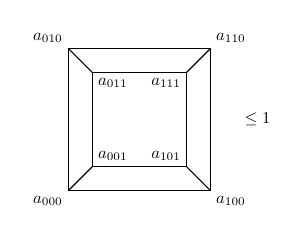
\begin{tikzpicture}[scale = 0.6, every node/.style = {scale = 0.6}]
                    \draw (0, 0) -- (3, 0) -- (3, 3) -- (0, 3) -- cycle;
                    \draw (0.5, 0.5) -- (2.5, 0.5) -- (2.5, 2.5) -- (0.5, 2.5) -- cycle;
                    \draw (0, 0) -- (0.5, 0.5);
                    \draw (3, 0) -- (2.5, 0.5);
                    \draw (3, 3) -- (2.5, 2.5);
                    \draw (0, 3) -- (0.5, 2.5);
                    \node[below left]  at (0, 0) {$a_{000}$};
                    \node[below right] at (3, 0) {$a_{100}$};
                    \node[above right] at (3, 3) {$a_{110}$};
                    \node[above left]  at (0, 3) {$a_{010}$};

                    \node[above right] at (0.5, 0.5) {$a_{001}$};
                    \node[above left]  at (2.5, 0.5) {$a_{101}$};
                    \node[below left]  at (2.5, 2.5) {$a_{111}$};
                    \node[below right] at (0.5, 2.5) {$a_{011}$};

                    \node at (4, 1.5) {$\le 1$};
                \end{tikzpicture}
            \end{center}
        \end{itemize}
    \end{column}

\end{columns}
\end{frame}